\usetikzlibrary{shapes.geometric, positioning}

\begin{ganttchart}[
    hgrid,
    vgrid,
    x unit=0.58cm,
    y unit title=0.5cm,
    y unit chart=0.53cm,
    title label font=\sffamily\footnotesize,
    bar label font=\sffamily\footnotesize,
    group label font=\sffamily\bfseries\footnotesize,
    milestone label font=\sffamily\footnotesize\itshape,
    bar label node/.append style={align=right, text width=7.3cm},
    group label node/.append style={align=right, text width=7.3cm},
    milestone label node/.append style={align=right, text width=6.8cm},
    bar/.style={fill=gray!30, rounded corners=2pt},
    group/.style={fill=gray!75},
    group peaks tip position=0,
    milestone/.style={fill=black, shape=diamond, scale=0.7},
    title height=1
]{1}{20}

  \gantttitle{Cronograma del Proyecto}{20} \\
  \gantttitle{Meses}{20} \\
  \gantttitle{1}{4}\gantttitle{2}{4}\gantttitle{3}{4}
  \gantttitle{4}{4}\gantttitle{5}{4} \\
  \gantttitle{Semanas}{20} \\
  \gantttitle{1}{1}\gantttitle{2}{1}\gantttitle{3}{1}\gantttitle{4}{1}
  \gantttitle{5}{1}\gantttitle{6}{1}\gantttitle{7}{1}\gantttitle{8}{1}
  \gantttitle{9}{1}\gantttitle{10}{1}\gantttitle{11}{1}\gantttitle{12}{1}
  \gantttitle{13}{1}\gantttitle{14}{1}\gantttitle{15}{1}\gantttitle{16}{1}
  \gantttitle{17}{1}\gantttitle{18}{1}\gantttitle{19}{1}\gantttitle{20}{1} \\

  % FASE 1 — secuencial
  \ganttgroup[group/.style={fill=gray!75}]{Fase 1 - Fundamentación}{1}{4} \\
  \ganttbar[bar/.style={fill=gray!30, rounded corners=2pt}]{Revisión literatura y antecedentes}{1}{2} \\
  \ganttbar[bar/.style={fill=gray!30, rounded corners=2pt}]{Análisis de soluciones existentes}{2}{3} \\
  \ganttbar[bar/.style={fill=gray!30, rounded corners=2pt}]{Estudio Hexagonal y DDD}{2}{3} \\
  \ganttbar[bar/.style={fill=gray!30, rounded corners=2pt}]{Revisión BIAN e ISO 20022}{3}{4} \\
  \ganttbar[bar/.style={fill=gray!30, rounded corners=2pt}]{Definición del marco de referencia}{4}{4} \\
  \ganttbar[bar/.style={fill=teal!25, rounded corners=2pt}]{Revisión y ajuste con el director}{2}{4} \\
  \ganttmilestone{Entrega: Marco de referencia documentado}{4} \\[grid]

  % FASE 2 — iterativa
  \ganttgroup[group/.style={fill=teal!60}]{Fase 2 - Mecanismo de generación}{5}{11} \\
  \ganttbar[bar/.style={fill=teal!25, rounded corners=2pt}]{Definición de requisitos y parámetros}{5}{6} \\
  \ganttbar[bar/.style={fill=teal!25, rounded corners=2pt}]{Diseño de la estructura modular base}{6}{7} \\
  \ganttbar[bar/.style={fill=teal!25, rounded corners=2pt}]{Construcción del mecanismo de generación}{7}{10} \\
  \ganttbar[bar/.style={fill=teal!25, rounded corners=2pt}]{Configuración del entorno reproducible}{8}{10} \\
  \ganttbar[bar/.style={fill=teal!25, rounded corners=2pt}]{Generación automática de documentación API}{10}{11} \\
  \ganttbar[bar/.style={fill=teal!25, rounded corners=2pt}]{Revisión y ajuste con el director}{6}{11} \\
  \ganttmilestone{Entrega: Mecanismo de generación}{11} \\[grid]

  % FASE 3 — iterativa
  \ganttgroup[group/.style={fill=teal!60}]{Fase 3 - Sistema de composición modular}{10}{16} \\
  \ganttbar[bar/.style={fill=teal!25, rounded corners=2pt}]{Identificación de funcionalidades reutilizables}{10}{11} \\
  \ganttbar[bar/.style={fill=teal!25, rounded corners=2pt}]{Definición de contratos y reglas de composición}{11}{12} \\
  \ganttbar[bar/.style={fill=teal!25, rounded corners=2pt}]{Implementación del sistema modular}{12}{15} \\
  \ganttbar[bar/.style={fill=teal!25, rounded corners=2pt}]{Validación con estándares BIAN e ISO 20022}{15}{16} \\
  \ganttbar[bar/.style={fill=teal!25, rounded corners=2pt}]{Revisión y ajuste con el director}{11}{16} \\
  \ganttmilestone{Entrega: Sistema de composición modular}{16} \\[grid]

  % FASE 4 — secuencial
  \ganttgroup[group/.style={fill=gray!75}]{Fase 4 - Evaluación y validación}{16}{20} \\
  \ganttbar[bar/.style={fill=gray!30, rounded corners=2pt}]{Definición de criterios de evaluación}{16}{17} \\
  \ganttbar[bar/.style={fill=gray!30, rounded corners=2pt}]{Aplicación en caso de estudio}{17}{18} \\
  \ganttbar[bar/.style={fill=gray!30, rounded corners=2pt}]{Recolección y análisis de datos}{18}{19} \\
  \ganttbar[bar/.style={fill=gray!30, rounded corners=2pt}]{Elaboración del informe de evaluación}{19}{20} \\
  \ganttbar[bar/.style={fill=teal!25, rounded corners=2pt}]{Revisión y ajuste con el director}{19}{20} \\
  \ganttmilestone{Entrega: Informe de evaluación}{20} \\[grid]

  % Transversal
  \ganttgroup[group/.style={fill=gray!75}]{Redacción documento final}{3}{20} \\

  % Leyenda
  \node[anchor=north east, inner sep=6pt, draw=gray!60, fill=white, line width=0.4pt] at ([xshift=-0.1cm, yshift=-2.7cm]current bounding box.north east) {%
    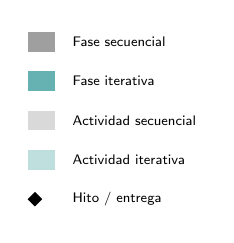
\begin{tikzpicture}
      \foreach \y/\col/\lbl in {
        0/gray!75/{Fase secuencial},
        0.50/teal!60/{Fase iterativa},
        1.00/gray!30/{Actividad secuencial},
        1.50/teal!25/{Actividad iterativa}
      }{
        \node[draw=none, fill=\col, minimum width=0.35cm, minimum height=0.25cm, anchor=west] at (0,-\y) {};
        \node[anchor=west, font=\sffamily\tiny] at (0.45,-\y) {\lbl};
      }
      \node[diamond, draw=none, fill=black, scale=0.4, anchor=west] at (0,-2.00) {};
      \node[anchor=west, font=\sffamily\tiny] at (0.45,-2.00) {Hito / entrega};
    \end{tikzpicture}
  };

\end{ganttchart}

\label{fig:gantt}